%
% Modified by Megan Patnott
% Last Change: Jan 18, 2013
%
%%%%%%%%%%%%%%%%%%%%%%%%%%%%%%%%%%%%%%%%%%%%%%%%%%%%%%%%%%%%%%%%%%%%%%%%
%
% Modified by Sameer Vijay
% Last Change: Tue Jul 26 2005 13:00 CEST
%
%%%%%%%%%%%%%%%%%%%%%%%%%%%%%%%%%%%%%%%%%%%%%%%%%%%%%%%%%%%%%%%%%%%%%%%%
%
% Sample Notre Dame Thesis/Dissertation
% Using Donald Peterson's ndthesis classfile
%
% Written by Jeff Squyres and Don Peterson
%
% Provided by the Information Technology Committee of
%   the Graduate Student Union
%   http://www.gsu.nd.edu/
%
% Nothing in this document is serious except the format.  :-)
%
% If you have any suggestions, comments, questions, please send e-mail
% to: ndthesis@gsu.nd.edu
%
%%%%%%%%%%%%%%%%%%%%%%%%%%%%%%%%%%%%%%%%%%%%%%%%%%%%%%%%%%%%%%%%%%%%%%%%


%
% Chapter 1
%

\chapter{INTRODUCTION}
Air travel in the U.S. is steadily growing due in part to an improving economy. Landings and take-offs at airports with FAA-operated towers and FAA-contracted towers are forecasted to increase from 48.9M to 59.9M or 22.5\% between 2015 and 2035 \cite{faa2015}. With the continuing growth of air traffic, additional airports are being built and existing airports are expanding. As this occurs, it is hard to ignore a significant byproduct: the increase in aircraft noise.

The steady encroachment of airports is especially problematic in metropolitan areas, where aircraft noise can negatively impact quality of life. While this issue began as a public interest initiative, a recent study has found a statistically significant link between aircraft noise and cardiovascular disease \cite{correia2013}. Correia et al. looked at 89 of the largest airports across the U.S., and found that, even when controlling for other environmental factors, a 10 dB increase in noise was associated with a 3.5 \% increase in hospital admissions in patients 65 years and older. Additional studies are ongoing, especially in the UK and EU, examining other potential adverse health effects such as delayed cognitive development in children,  \cite{cap2014}. In light of these studies, it is clear: engineers and scientists have an ethical imperative to ensure the safety of technology. 

Progress is being made in the field of aeroacoustics. In general, aircraft have become ``quieter'', especially due to the widespread adoption of the turbofan jet engine. With the reduction of jet engine noise, aircraft noise has come to a level comparable to that of the airframe on approach and landing conditions \cite{dob2010}. The airframe is the new ``lower noise barrier'' of aircraft noise production. Efforts have been taken to quantify airframe noise. Gibson performed flyover noise measurements and identified landing gears and high-lift devices as the two major noise contributors \cite{gibson}.

In addition to these efforts, several government initiatives have been launched to advance quiet aircraft technology. In the EU, European Visions 2020 requires to ``reduce subjective noise impact by half'' (minus 10 dB) per operation by 2020 relative to year 2000 level technology \cite{dob}. While in the US, the national Advanced Subsonic Transport (AST) and Quiet Aircraft Technology research programs have even more stringent milestones.

Due in part to these initiatives, many basic noise reduction technologies have been applied to aircraft landing gear. 

Dobrzynski et al. studied the effect of solid, streamlined add-on fairings to various areas of main and nose landing gears. While these fairings were effective at reducing mid and high frequency noise levels, they also had adverse effects. This study and those like it revealed that solid fairings acted to increase local flow velocity and thereby noise from adjacent gear components.

The findings of solid fairing studies suggested that if flow could be 
Ravetta et al. Porous fairings

These technologies utilize passive flow control. 

This study is focused on the application of active flow control.

\section{Motivation}
The present work is motivated to reduce noise produced by aircraft landing gear by flow control via application of DBD plasma actuators. To this end, experiments will be performed to 
1) better understand the noise generation mechanisms present on aircraft landing gear, thereby aiding in the formation of flow control strategies.
2) Take steps toward the development of ``plasma fairing'' technology, which is a device that can be retrofitted to existing aircraft landing gears with the purpose of reducing noise production.


In this chapter, the physics of airframe noise production are discussed. The structure of Aircraft landing gear is presented. This geometry is grouped into two main sub-systems and flow control strategies are recommended for both. Areas of noise contribution are considered and the underlying physical mechanisms are identified. Finally, the literature is reviewed with respect to the application of Plasma Flow Control to increasingly complex geometries.

\section{Theory of Aeroacoustics}
To arrive at a viable flow control strategy, it is useful to first review the underlying physics.
The modern theory of aeroacoustics, that is sound generated by aerodynamic means, is based on James Lighthill's so-called acoustic analogy. He states that sound generated in a fluid flow is only important in regions of turbulent fluctuations \cite{howe2003}. Based on this assumption, the Navier-Stokes Equation and isentropic equation of state in indicial notation are

\begin{equation} \label{eq:1-1}
	\frac{\partial \rho}{\partial t} + \frac{\partial(\rho u_i)}{\partial x_i} = 0,
\end{equation}

\begin{equation} \label{eq:1-2}
\frac{\partial (\rho u_i)}{\partial t} + \frac{\partial(\rho u_i u_j + P_{ij})}{\partial x_j} = 0,
\end{equation}

\begin{equation} \label{eq:1-3}
	c_o^2 = \frac{\partial p}{\partial \rho}|_{s=const.} = \frac{p'}{\rho'}
\end{equation}

where 

\begin{equation} \label{eq:pij}
P_{ij} = p' \delta_{ij} - \sigma_{ij}.
\end{equation}

$P_{ij}$ is the total stress tensor including pressure and viscous terms, $\rho$ is the fluid density, $u$ is  the local velocity vector, $p$ is the pressure and $c_o$ is the local speed of sound. Also, $p' = p - p_o$ and $\rho' = \rho - \rho_o$ represent the fluctuating pressure and density relative to the mean values, respectively. After assuming sufficiently small fluctuations, equations \ref{eq:1-1} and \ref{eq:1-2} can be linearized yielding the classical Lighthill's equation

\begin{equation} \label{eq:1-4}
\frac{\partial^2 \rho}{\partial t^2} - c_o^2 \nabla^2 \rho = \frac{\partial^2 T_{ij}}{\partial x_i \partial x_j},
\end{equation}

where the source term $T_{ij}$ is known as Lighthill's turbulence stress tensor

\begin{equation}
T_{ij} = \rho u_i u_j + P_{ij} - c_o^2(\rho - \rho_0) \delta_{ij},
\end{equation}

and where $\delta_{ij}$ is the Kronecker delta which is defined as,
\begin{equation}
\delta_{ij} = \left\{
\begin{array}{lcr}
1 & \mbox{if} & i = j \\
0 & \mbox{if} & i \neq j
\end{array}
\right\}.
\end{equation}

For the special case of high Reynolds number, incompressible flow, both the density fluctuations and the viscous stresses are negligible, reducing the Lighthill stress tensor to

\begin{equation}
T_{ij} \approx \rho_0 u_i u_j.
\end{equation}

Equation \ref{eq:1-4} can be solved and formulated in terms of $p'$ by combining with equation \ref{eq:1-3} giving

\begin{equation}
p' = c_o^2 \rho' = \frac{1}{4\pi} \frac{\partial^2}{\partial x_i \partial x_j} \int_{V} \frac{T_{ij}}{r}dV,
\end{equation}

where $V$ represents the volume of the region of interest, and $r$ represents the distance to the acoustic source.

In 1955, Lighthill's analogy was extended to account for the presence of solid boundaries within the turbulent flow region \cite{curle1955}.  The general solution to this equation is 

\begin{equation} \label{eq:1-9}
\begin{aligned}
p' &= \underbrace{ \frac{1}{4\pi} \frac{\partial^2}{\partial x_i \partial x_j} \int_V \left[ \frac{T_{ij}}{r} \right] dV }_I - \underbrace{ \frac{1}{4\pi} \frac{\partial}{\partial x_j} \int_S \left[ \frac{P_{ij} + \rho u_i u_j}{r} \right] n_i dS }_{II} \\
&+ \underbrace{ \frac{1}{4\pi} \frac{\partial}{\partial t} \int_S \left[ \frac{\rho u_i}{r} \right] n_i dS}_{III},
\end{aligned}
\end{equation}

where $S$ represents the control surface bounding the volumetric region of interest \cite{hirschberg2004}. Equation \ref{eq:1-9} forms the basis of airframe noise generation by including the effects of reflection and diffraction of acoustic waves at the boundaries.

To illustrate the nature of the acoustic source terms on the right hand side of equation \ref{eq:1-9}, an order-of-magnitude scaling analysis is performed with the purpose of determining the radiation patterns of the hypothetical acoustic source with respect to flow speed, $U_o$, and propagation distance, $r$. Lighthill conveniently used a subsonic, turbulent isothermal jet to define a physical application for which characteristic length, frequency, pressure scales, and velocity are defined \cite{lighthill1954}. Substituting the pertinent characteristic scales yields the following order-of-magnitude approximations for the components of the acoustic source term:

\begin{equation} \label{eq:D}
\int_{V} dV \propto D^3
\end{equation}

\begin{equation} \label{eq:U}
T_{ij} \propto \rho_o U_o^2
\end{equation}

\begin{equation} \label{eq:dx}
\frac{\partial}{\partial x_i} = \frac{\partial}{c_o \partial t} \propto \frac{f}{c_o} \propto \frac{U_o}{c_o D}
\end{equation}

Equations \ref{eq:D} - \ref{eq:dx} are then utilized to replace the source terms in equation \ref{eq:1-9}, resulting in the following:

\begin{equation}
I : \frac{1}{4\pi} \frac{\partial^2}{\partial x_i \partial x_j} \int_V \left[ \frac{T_{ij}}{r} \right] dV \propto \left( \frac{U_o}{c_o D} \right)^2 \left( D^3 \right) \left( \frac{\rho_o U_o^2}{r} \right) \propto \frac{U_o^4}{r},
\end{equation}

\begin{equation}
II : \frac{1}{4\pi} \frac{\partial}{\partial x_j} \int_S \left[ \frac{P_{ij} + \rho u_i u_j}{r} \right] n_i dS \propto \left( \frac{U_o}{c_oD} \right) \left( \frac{\rho_o U_o^2}{r} \right) \left( D^2 \right) \propto \frac{U_o^3}{r},
\end{equation}

\begin{equation}
III : \frac{1}{4\pi} \frac{\partial}{\partial t} \int_S \left[ \frac{\rho u_i}{r} \right] n_i dS \propto \left( \frac{U_o}{D} \right) \left( \frac{\rho_o U_o}{r} \right) \left( D^2 \right) \propto \frac{U_o^2}{r}.
\end{equation}

This analysis assumes that the freestream Mach number is much less than unity or $M = \frac{U_o}{c_o} << 1$, and that far-field acoustic radiation dominates the signal so that it acts as a spherically-spreading pressure wave. 

Furthermore, the radiated acoustic power $W$, is proportional to the square of the pressure field, giving

\begin{equation} \label{eq:u8}
I : W \propto p'^2 \propto \frac{U_o^8}{r^2},
\end{equation}

\begin{equation} \label{eq:u6}
II : W \propto p'^2 \propto \frac{U_o^6}{r^2},
\end{equation}

\begin{equation} \label{eq:u4}
III : W \propto p'^2 \propto \frac{U_o^4}{r^2}.
\end{equation}

The results of the scaling analysis presented in equation \ref{eq:u8} correspond physically to the radiation pattern of a volumetric distribution of quadrupole sources. Therefore, Lighthill's acoustic analogy states that the far-field acoustic pressure field of a region of turbulence in a steady flow, and  a region of quadrupole acoustic sources with no flow are equivalent. Similarly, equations \ref{eq:u6} and \ref{eq:u4} represent a distribution of dipole and monopole sources, respectively. Finally, this analysis shows that a decrease in acoustic power of the system corresponds to an increase in acoustic efficiency when transitioning from a quadrupole to a dipole to a monopole. These trends are extremely useful in determining the nature of the acoustic sources present in flows around complex geometries, such as around aircraft landing gears.

\section{Landing Gear}
As previously stated, aircraft landing gear have been identified as a primary source of airframe noise especially for the larger wide-body configurations \cite{}. 

Landing gear generally come in two types: nose landing gear (NLG) and main landing gear (MLG). The former is designed for steering while the latter is designed for braking. 

The scope of this study is limited to work on the G550 nose landing gear, but while many designs vary in each aircraft, it is probable that flow control strategies will overlap. 

\subsection{Geometry}

The Gulfstream G550 Nose landing gear was selected due to an industry collaboration with NASA. In Neuhart et al., this design was aerodynamically characterized to provide a database of aerodynamic and acoustic data by which to compare experiments and simulations. 

The actual landing gear is depicted in Figure \ref{fig:lg1} for reference, and shown schematically in Figure \ref{fig:lg2}.



\begin{figure}
	\begin{center}
		\centerline{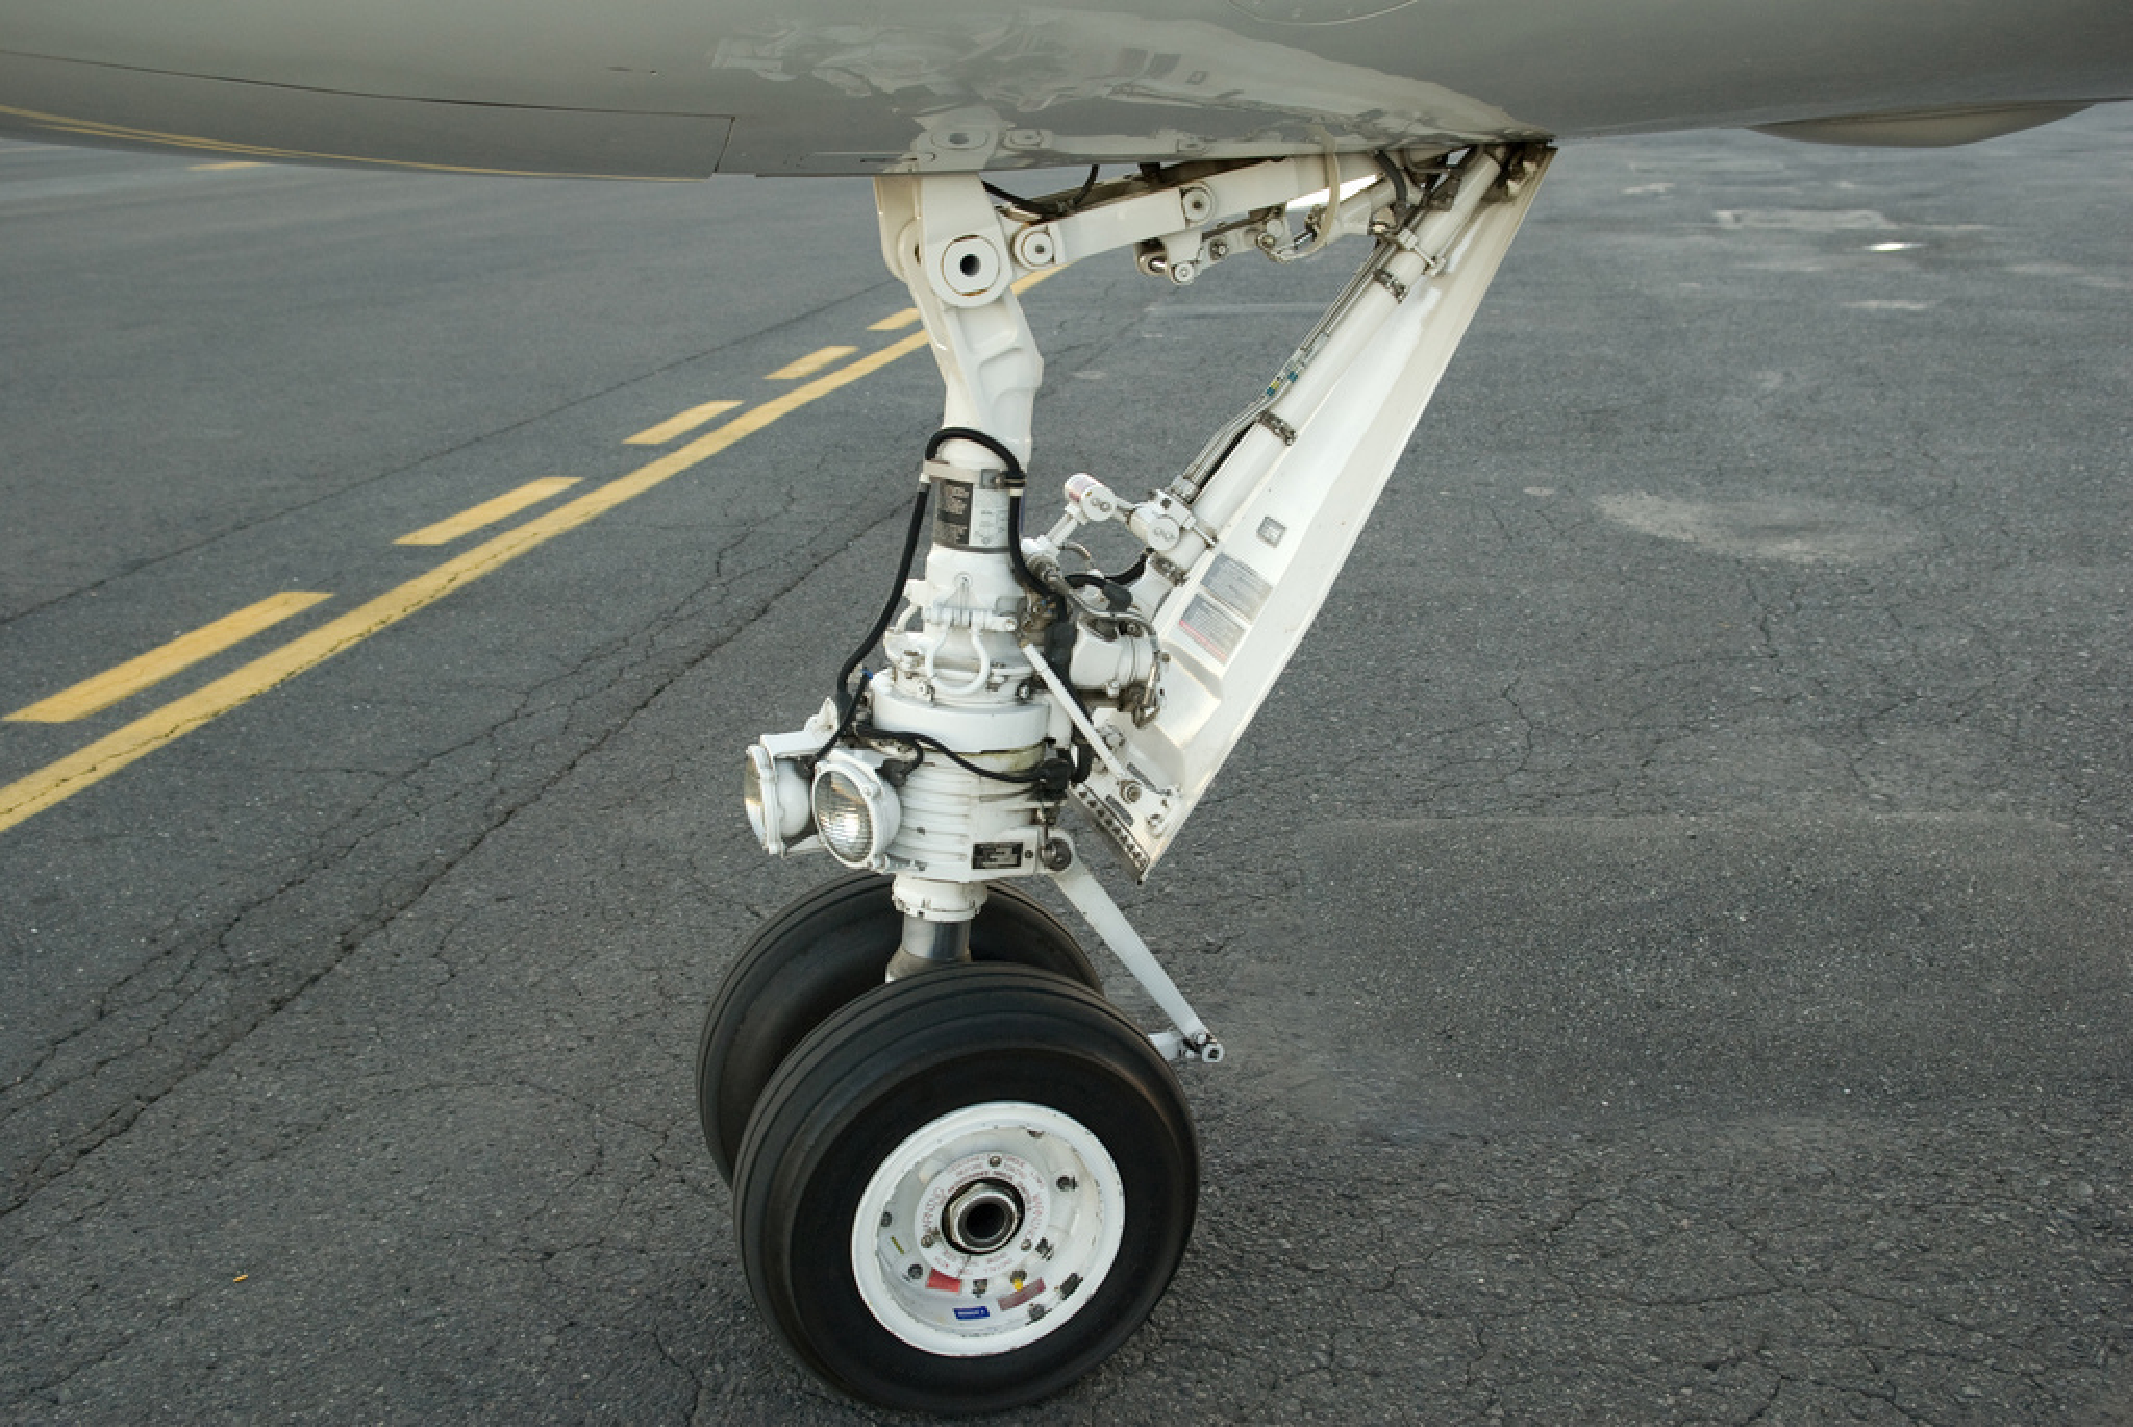
\includegraphics[scale=0.4]{figures/g550_nlg.pdf}}
		\caption{Photograph of Gulfstream 550 Nose Landing Gear.}
		\label{fig:lg1}
	\end{center}
\end{figure}

\begin{figure}
	\begin{center}
		\centerline{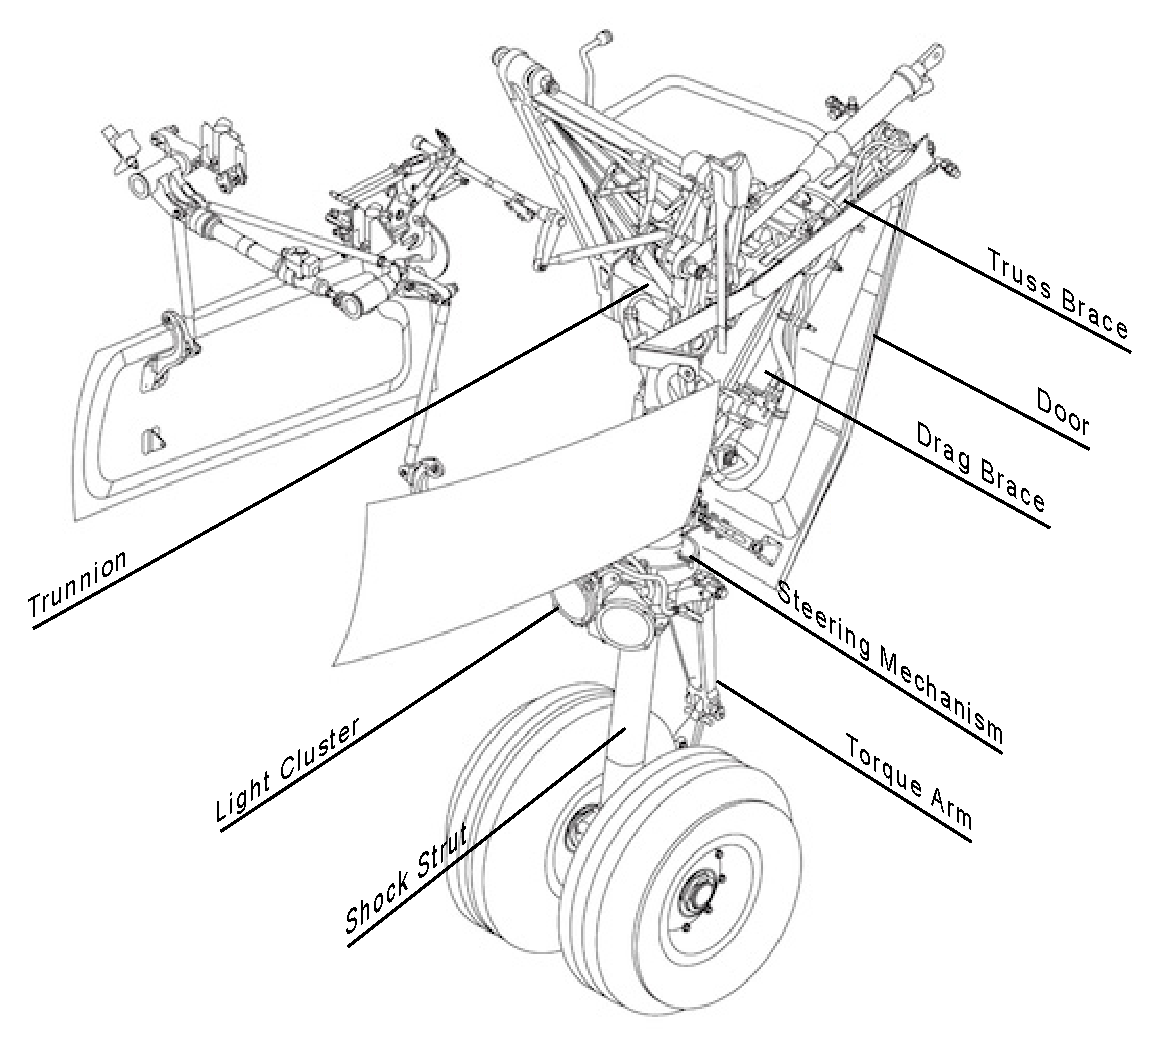
\includegraphics[scale=0.7]{figures/lg_schematic.pdf}}
		\caption{Schematic view of Gulfstream 550 Nose Landing Gear components.}
		\label{fig:lg2}
	\end{center}
\end{figure}


\subsection{Noise Sources}
Recall that adding a solid boundary to the flow drastically altered the source terms in equation \ref{eq:1-9}. In experiments, these terms manifest as flow-generated noise. Typically there are two types: 

\begin{itemize}  
        \item Tonal - generated by periodic flow events (such as vortex shedding),
        \item Broadband - generated by random flow events (such as turbulence). 
\end{itemize}
    
    Most aerodynamic bodies are characterized by their drag force. When a body is streamlined, it is said that the total drag is dominated by the viscous drag component.  However, for some bodies the total drag is dominated by the pressure drag component, these bodies are referred to as bluff. Bluff bodies can be a major contributor to flow-generated noise, due in part to the unsteady wake these structures tend to cause. The canonical example of a bluff body is a simple cylinder, for which the flow is well understood. It is dominated by large-scale von Karman vortex shedding of frequency $f$, over the cylinder body of characteristic length $L$. This vortex shedding frequency is characterized by the dimensionless Strouhal number $St = \frac{fL}{U_\infty}$, which is constant over a wide range of Reynolds numbers $Re = \frac{\rho U_\infty L}{\mu}$ \cite{bearman1969}, where $\rho$ and $\mu$ represent mean density and dynamic viscosity of the freestream flow, respectively. This large-scale vortex shedding corresponds to periodic unsteady surface pressure which is responsible for the generation of tonal noise. 
    
More complex geometries such as the landing gear, can be considered as a collections of bluff bodies. Counter-intuitively, the acoustic signature for the landing gear is broadband in nature which is associated with turbulence \cite{astley2008}. As depicted in Figure \ref{fig:lg1}, the landing gear components are arranged in close proximity to one another. It is possible that this proximity stifles full wake development, effectively preventing the large-scale vortex shedding observed for the simple cylinder. This suggests that flow control on fundamental geometries, while useful, may not be representative of the actual flow physics. This is the foundation for the previously suggested strategy of examining sub-systems. 

In addition to varying inter-component spacings, the presence of multiple length scales in the landing gear geometry implies that some components may also contribute to the total noise as reflective sources. Guo et al. divided the far-field noise propagation into three regimes based on the concept of acoustic compactness \cite{guo2006} Since an acoustic wave in a medium is governed by the speed of sound then $c_o = \lambda f$. A source is said to be acoustically compact if $kL << 1$ where $k$ is the acoustic wavenumber defined as $k = \frac{2 \pi}{\lambda} = \frac{2 \pi f}{c_o}$, $\lambda$ is the acoustic wavelength, and $L$ is the characteristic length. It is noncompact if $kL \geq 1$. For a full-scale Boeing 737 main landing gear large (wheels and doors) and medium geometries (main struts and linkages) represented low and mid-range frequencies, respectively. Small geometries (hoses, sharp edges, and electrical wiring) represented high frequency noncompact acoustic sources. While compact sources behave like a distribution of dipoles, noncompact sources represent phase variations in surface pressure leading to degradation of radiation efficiency (quadrupole). 

Before discussing a strategy for flow control, it is useful to first consider the physical phenomena present. While quantifying the contribution of each mechanism to the total acoustic signature of the landing gear, is a fairly difficult task, an order-of-magnitude analysis can be applied to estimate a potential dominant source. Table \ref{tab:source} lists the sources considered, corresponding acoustic power, noise type, and source type. Recall that high acoustic power corresponds to low acoustic efficiency, meaning a monopole source is a more effective noise producer than a quadrupole source. Focusing on the more efficient dipole sources present, the mechanisms of unsteady wake and downstream wake impingement are the most viable candidates for flow control. Vortex shedding may be present but is highly tonal, and the broadband nature of landing gear noise suggests that this is probably a minor noise producer.

\begin{table}
 \setlength{\capwidth}{0.7\textwidth}
\begin{center}
\caption{Physical mechanisms of flow-generated noise.}
\label{tab:source}
\begin{tabular}{llll}\toprule
\parbox{0.15\linewidth}{Mechanism} & 
\parbox{0.15\linewidth}{Acoustic Power} & 
\parbox{0.15\linewidth}{Source Type} & 
\parbox{0.15\linewidth}{Noise Type} \\ \midrule
Vortex Shedding & $\frac{U_o^6}{r^2}$ & Dipole & Tonal  \\
Wake Shear Layer & $\frac{U_o^8}{r^2}$ & Quadrupole & Broadband \\
Wake Turbulence & $\frac{U_o^8}{r^2}$ & Quadrupole & Broadband \\
Downstream Wake Impingement & $\frac{U_o^6}{r^2}$ & Dipole & Broadband \\
Unsteady Wake & $\frac{U_o^6}{r^2}$ & Dipole & Broadband \\
Reflective Sources & $\frac{U_o^8}{r^2}$ & Quadrupole & Tonal or Broadband \\ \bottomrule
\end{tabular}
\end{center}
\end{table}


These physical phenomena are considered in the following review of literature.

\section{Literature Review}

This section provides a review of aeroacoustic research pertinent to the development of a plasma fairing 

\subsection{Single Cylinder Plasma Flow Control}

The single cylinder is the most simplified representation of the landing gear strut. Active flow control efforts by means of DBD plasma actuators were first applied to this generic bluff body geometry as proof-of-concept. Several experiments and large-eddy simulations (LES) were performed at the University of Notre Dame to show the viability of this technology \cite{kozlov2009}. Two flow control strategies were employed: spanwise plasma actuators, and plasma streamwise vortex generators (PSVGs). The latter of these devices is made up of a spanwise array of electrodes oriented in the streamwise direction. Flow visualization of these techniques is shown in Figure \ref{fig:flowvis}. 

Both approaches were effective in significantly suppressing Karman vortex shedding, if by different mechanisms. Spanwise plasma actuators achieve flow control through modification of the detached free shear layer. PSVGs induce streawise voriticity into the nascent cylinder wake, promoting rapid wake mixing. Kozlov et al. performed near field microphone measurements with $d=$ 0.61 m, demonstrating a reduction in noise levels of 11.2 dB and 14.2 dB for spanwise actuators and PSVGs, respectively. These results were promising and inspired more studies on a slightly more complex geometry: tandem cylinders.

\begin{figure}
	\begin{center}
		\centerline{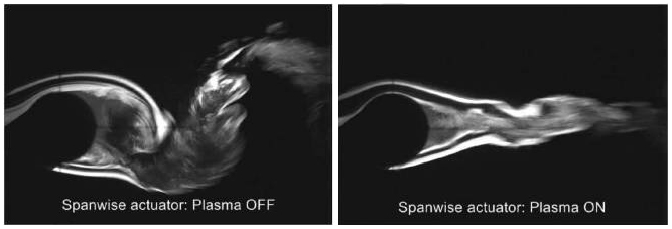
\includegraphics[scale=1.0]{figures/single_span.pdf}}
		\centerline{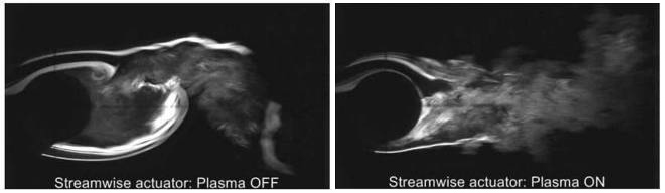
\includegraphics[scale=1.0]{figures/single_psvg.pdf}}
		\caption{Flow Visualization of single cylinder in cross-flow with Spanwise and PSVG plasma actuators.}
		\label{fig:cyl1}
	\end{center}
\end{figure}


\subsection{Tandem Cylinders Plasma Flow Control}

The tandem cylinders configuration is the next stage in the development of flow control for aircraft landing gear. The interaction between the two bluff bodies represents that between main strut and downstream components. 

Zdravkovich comprehensively reviewed two circular cylinders of the same diameter at subcritical Reynolds number. 

\cite{zdrovkovich}

\cite{kozlov}
\cite{khorami}
\cite{wang}






\begin{figure}
	\begin{center}
		\centerline{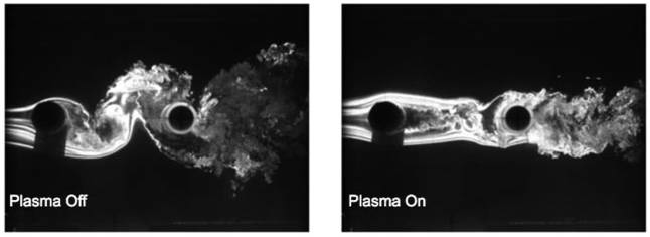
\includegraphics[scale=1.0]{figures/tandem_span}}
		\centerline{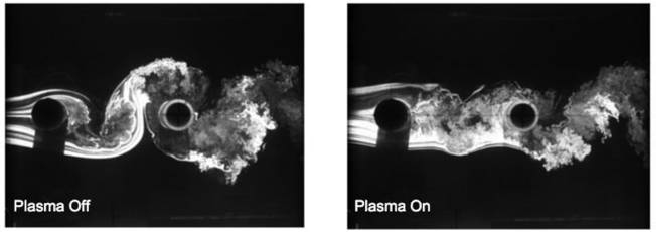
\includegraphics[scale=1.0]{figures/tandem_psvg}}
		\caption{Flow Visualization of tandem cylinders in cross-flow with Spanwise and PSVG plasma actuators.}
		\label{fig:cyl2}
	\end{center}
\end{figure}

\subsection{Shock Strut-Torque Arm Assembly Plasma Flow Control}

Huang et al. studied the acoustic of plasma actuators on a torque arm apparatus. By applying spanwise plasma actuators in both an 'upstream' and 'downstream' configuration, two types of flow control were explored. The upstream configuration served to create a virtual plasma fairing effect by routing the shear layers around the downstream components, reducing the overall noise generated by wake impingement. The downstream configuration is shown to have reduced vortical structures, lowering the unsteadiness int he wake. 
\cite{huang1}
\cite{huang2}

\begin{figure}
	\begin{center}
		\centerline{\includegraphics[scale=1.0]{figures/torque_arm}}
		\caption{Flow Visualization of torque-arm assembly in cross-flow with Spanwise plasma actuators.}
		\label{fig:cyl2}
	\end{center}
\end{figure}


%Table~\ref{tbl:bogus1} shows some feeding frequencies for where Gnus
%like to eat around the Notre Dame campus.  Gnus have work weeks, just
%like humans do, hence the much lower frequencies on weekends.  This
%can lead us to conclude that Gnu weekend shifts are much smaller than
%the normal work-week shifts.  In fact, we can attempt to parametrize the
%sighting frequency, $\mathcal{F}$, by the student population, type of food, and
%day of the week as:
%\begin{equation}
%  \mathcal{F} = \mathcal{F}(p,f,d).
%\end{equation}
%Table~\ref{tbl:bogus2} shows what they
%typically like to eat.
%
%\begin{table}[tpb]
%  \begin{center}
%    \caption{WHERE Gnus LIKE TO EAT \label{tbl:bogus1}}
%    \begin{tabularx}{0.85\textwidth}{lrrrrrrr} \toprule
%      \multicolumn{1}{c}{Location} & Sun & Mon & Tue & Wed & Thu & Fri & Sat \\ \midrule
%      Front of Dome & 1 & 5 & 6 & 5 & 4 & 5 & 1 \\
%      Stonehenge & 2 & 9 & 10 & 12 & 9 & 14 & 2 \\
%      The Rock & 1 & 3 & 4 & 3 & 4 & 3 & 0 \\
%      The ACC & 3 & 4 & 5 & 5 & 5 & 4 & 1 \\
%      Dining Halls & 5 & 14 & 12 & 13 & 14 & 12 & 3 \\
%      Hesburgh Library & 2 & 3 & 5 & 2 & 3 & 4 & 2 \\ \bottomrule
%    \end{tabularx}
%  \end{center}
%\end{table}
%
%\begin{table}[tpb]
%  \setlength{\capwidth}{0.7\textwidth}
%  \begin{center}
%    \caption{WHAT Gnus LIKE TO EAT ON THE NOTRE DAME CAMPUS, LISTED
%      BY AVERAGE NUMBER OF SIGHTINGS PER WEEKDAY
%    \label{tbl:bogus2}
%}
%    \begin{tabular}{lrrrrrrr} \toprule
%      \multicolumn{1}{c}{Food} & Sun & Mon & Tue & Wed & Thu & Fri & Sat \\ \midrule
%      Twinkies & 1 & 5 & 6 & 5 & 4 & 5 & 1 \\
%      Ding Dongs & 2 & 9 & 10 & 12 & 9 & 14 & 2 \\
%      Carrots & 1 & 3 & 4 & 3 & 4 & 3 & 0 \\
%      Lettuce & 3 & 4 & 5 & 5 & 5 & 4 & 1 \\
%      Twizlers & 5 & 14 & 12 & 13 & 14 & 12 & 3 \\
%      Jawbreakers & 2 & 3 & 5 & 2 & 3 & 4 & 2 \\ \bottomrule
%    \end{tabular}
%  \end{center}
%\end{table}
%
%Figure~\ref{fig:bogus3} shows a nice graph of location distributions
%by day of week.  I have no real reason for including it except to show
%that figures work as well.  Did I mention that Gnus are really cool?
%
%\begin{figure}[tpb]
%  \begin{center}
%    \centerline{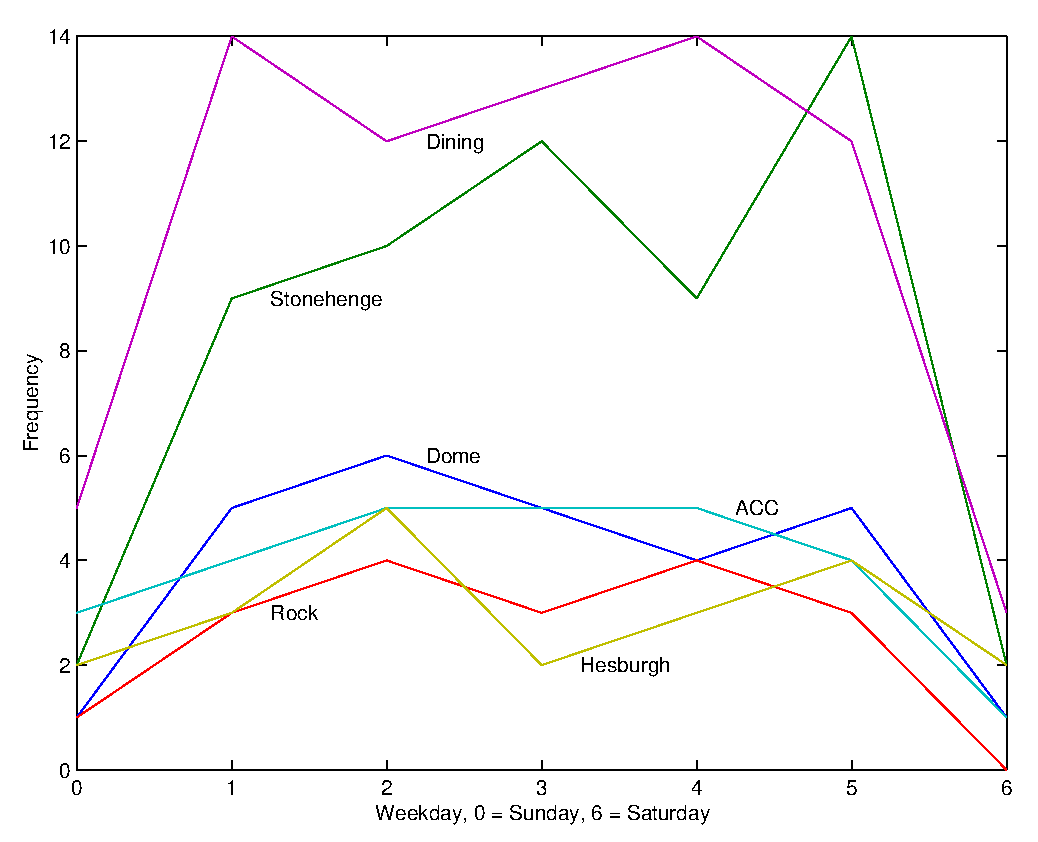
\includegraphics[scale=0.8]{sample_nd}}
%    \caption{Location distributions by day of where, where the X axis
%      is the weekday (0 through 6), and the Y axis is the sighting
%      frequency}
%    \label{fig:bogus3}
%  \end{center}
%\end{figure}
%
%Gnus typically tend to come out when there are large gatherings of
%humans with food.  Gnus work very hard at providing us with all the
%things that we like (trees, dirt, air, etc.), and so we should freely
%give them food.  They will come up and stand a respectful distance
%away from you, waiting to see if they will be rewarded for their
%efforts.  If you offer some food, they will take it and back off a
%respectful distance in order to consume their food while leaving you
%to your ``personal space.''

%\section{Groovin' Gnus}
%\label{sec:groovin-gnus}
%
%Gnus do tend to stay away from humans in their normal day-to-day
%workings.  This is mainly because humans don't, for the most part,
%understand what they are doing.  If a Gnu is working, and a human
%approaches it, the Gnu will tend to drop whatever it is doing and run
%away.  This is probably do to the tendency for humans to have ``group
%meetings'' and ``productivity seminars.''  Most Gnus are deathly
%afraid of such overmanagement, and run at the slightest hint of it,
%for fear that it will cripple their real work.
%
%It is interesting, however, that Gnus have chosen an Institution of
%Higher Education for their BOO.\footnote{Base of Operations.}  It is
%often said that:
%\begin{quote}
%  Academic politics are the dirtiest, meanest, ugliest, and generally
%  the most low-down, in-your-face, and kick-em-while-they're-down than
%  anywhere else (even Washington D.C.)  because the stakes are so low.
%\end{quote}
%It has been hypothesized that the Gnus are subtly trying to affect a
%change for the better (i.e., eliminating the overmanagement problems)
%by working the very system that they are trying to change, from
%within.  That is, the graduates from Notre Dame can learn from the
%examples of the Gnus here, and run screaming (or chattering) at the
%slightest hint of overmanagement, and let the real work proceed
%unhindered.

% % uncomment the following lines,
% if using chapter-wise bibliography
%
% \bibliographystyle{ndnatbib}
% \bibliography{example}
